% Options for packages loaded elsewhere
\PassOptionsToPackage{unicode}{hyperref}
\PassOptionsToPackage{hyphens}{url}
%
\documentclass[
]{article}
\usepackage{amsmath,amssymb}
\usepackage{lmodern}
\usepackage{iftex}
\ifPDFTeX
  \usepackage[T1]{fontenc}
  \usepackage[utf8]{inputenc}
  \usepackage{textcomp} % provide euro and other symbols
\else % if luatex or xetex
  \usepackage{unicode-math}
  \defaultfontfeatures{Scale=MatchLowercase}
  \defaultfontfeatures[\rmfamily]{Ligatures=TeX,Scale=1}
\fi
% Use upquote if available, for straight quotes in verbatim environments
\IfFileExists{upquote.sty}{\usepackage{upquote}}{}
\IfFileExists{microtype.sty}{% use microtype if available
  \usepackage[]{microtype}
  \UseMicrotypeSet[protrusion]{basicmath} % disable protrusion for tt fonts
}{}
\makeatletter
\@ifundefined{KOMAClassName}{% if non-KOMA class
  \IfFileExists{parskip.sty}{%
    \usepackage{parskip}
  }{% else
    \setlength{\parindent}{0pt}
    \setlength{\parskip}{6pt plus 2pt minus 1pt}}
}{% if KOMA class
  \KOMAoptions{parskip=half}}
\makeatother
\usepackage{xcolor}
\usepackage[margin=1in]{geometry}
\usepackage{color}
\usepackage{fancyvrb}
\newcommand{\VerbBar}{|}
\newcommand{\VERB}{\Verb[commandchars=\\\{\}]}
\DefineVerbatimEnvironment{Highlighting}{Verbatim}{commandchars=\\\{\}}
% Add ',fontsize=\small' for more characters per line
\usepackage{framed}
\definecolor{shadecolor}{RGB}{248,248,248}
\newenvironment{Shaded}{\begin{snugshade}}{\end{snugshade}}
\newcommand{\AlertTok}[1]{\textcolor[rgb]{0.94,0.16,0.16}{#1}}
\newcommand{\AnnotationTok}[1]{\textcolor[rgb]{0.56,0.35,0.01}{\textbf{\textit{#1}}}}
\newcommand{\AttributeTok}[1]{\textcolor[rgb]{0.77,0.63,0.00}{#1}}
\newcommand{\BaseNTok}[1]{\textcolor[rgb]{0.00,0.00,0.81}{#1}}
\newcommand{\BuiltInTok}[1]{#1}
\newcommand{\CharTok}[1]{\textcolor[rgb]{0.31,0.60,0.02}{#1}}
\newcommand{\CommentTok}[1]{\textcolor[rgb]{0.56,0.35,0.01}{\textit{#1}}}
\newcommand{\CommentVarTok}[1]{\textcolor[rgb]{0.56,0.35,0.01}{\textbf{\textit{#1}}}}
\newcommand{\ConstantTok}[1]{\textcolor[rgb]{0.00,0.00,0.00}{#1}}
\newcommand{\ControlFlowTok}[1]{\textcolor[rgb]{0.13,0.29,0.53}{\textbf{#1}}}
\newcommand{\DataTypeTok}[1]{\textcolor[rgb]{0.13,0.29,0.53}{#1}}
\newcommand{\DecValTok}[1]{\textcolor[rgb]{0.00,0.00,0.81}{#1}}
\newcommand{\DocumentationTok}[1]{\textcolor[rgb]{0.56,0.35,0.01}{\textbf{\textit{#1}}}}
\newcommand{\ErrorTok}[1]{\textcolor[rgb]{0.64,0.00,0.00}{\textbf{#1}}}
\newcommand{\ExtensionTok}[1]{#1}
\newcommand{\FloatTok}[1]{\textcolor[rgb]{0.00,0.00,0.81}{#1}}
\newcommand{\FunctionTok}[1]{\textcolor[rgb]{0.00,0.00,0.00}{#1}}
\newcommand{\ImportTok}[1]{#1}
\newcommand{\InformationTok}[1]{\textcolor[rgb]{0.56,0.35,0.01}{\textbf{\textit{#1}}}}
\newcommand{\KeywordTok}[1]{\textcolor[rgb]{0.13,0.29,0.53}{\textbf{#1}}}
\newcommand{\NormalTok}[1]{#1}
\newcommand{\OperatorTok}[1]{\textcolor[rgb]{0.81,0.36,0.00}{\textbf{#1}}}
\newcommand{\OtherTok}[1]{\textcolor[rgb]{0.56,0.35,0.01}{#1}}
\newcommand{\PreprocessorTok}[1]{\textcolor[rgb]{0.56,0.35,0.01}{\textit{#1}}}
\newcommand{\RegionMarkerTok}[1]{#1}
\newcommand{\SpecialCharTok}[1]{\textcolor[rgb]{0.00,0.00,0.00}{#1}}
\newcommand{\SpecialStringTok}[1]{\textcolor[rgb]{0.31,0.60,0.02}{#1}}
\newcommand{\StringTok}[1]{\textcolor[rgb]{0.31,0.60,0.02}{#1}}
\newcommand{\VariableTok}[1]{\textcolor[rgb]{0.00,0.00,0.00}{#1}}
\newcommand{\VerbatimStringTok}[1]{\textcolor[rgb]{0.31,0.60,0.02}{#1}}
\newcommand{\WarningTok}[1]{\textcolor[rgb]{0.56,0.35,0.01}{\textbf{\textit{#1}}}}
\usepackage{longtable,booktabs,array}
\usepackage{calc} % for calculating minipage widths
% Correct order of tables after \paragraph or \subparagraph
\usepackage{etoolbox}
\makeatletter
\patchcmd\longtable{\par}{\if@noskipsec\mbox{}\fi\par}{}{}
\makeatother
% Allow footnotes in longtable head/foot
\IfFileExists{footnotehyper.sty}{\usepackage{footnotehyper}}{\usepackage{footnote}}
\makesavenoteenv{longtable}
\usepackage{graphicx}
\makeatletter
\def\maxwidth{\ifdim\Gin@nat@width>\linewidth\linewidth\else\Gin@nat@width\fi}
\def\maxheight{\ifdim\Gin@nat@height>\textheight\textheight\else\Gin@nat@height\fi}
\makeatother
% Scale images if necessary, so that they will not overflow the page
% margins by default, and it is still possible to overwrite the defaults
% using explicit options in \includegraphics[width, height, ...]{}
\setkeys{Gin}{width=\maxwidth,height=\maxheight,keepaspectratio}
% Set default figure placement to htbp
\makeatletter
\def\fps@figure{htbp}
\makeatother
\setlength{\emergencystretch}{3em} % prevent overfull lines
\providecommand{\tightlist}{%
  \setlength{\itemsep}{0pt}\setlength{\parskip}{0pt}}
\setcounter{secnumdepth}{-\maxdimen} % remove section numbering
\ifLuaTeX
  \usepackage{selnolig}  % disable illegal ligatures
\fi
\IfFileExists{bookmark.sty}{\usepackage{bookmark}}{\usepackage{hyperref}}
\IfFileExists{xurl.sty}{\usepackage{xurl}}{} % add URL line breaks if available
\urlstyle{same} % disable monospaced font for URLs
\hypersetup{
  pdftitle={Process data from reproducibility service},
  pdfauthor={Lars Vilhuber},
  hidelinks,
  pdfcreator={LaTeX via pandoc}}

\title{Process data from reproducibility service}
\author{Lars Vilhuber}
\date{2023-05-24}

\begin{document}
\maketitle

{
\setcounter{tocdepth}{2}
\tableofcontents
}
\begin{quote}
Note: The
\href{https://aeadataeditor.github.io/processing-jira-process-data/README.pdf}{PDF
version} of this document is transformed by manually printing from a
browser.
\end{quote}

\hypertarget{citation}{%
\subsection{Citation}\label{citation}}

\begin{quote}
Vilhuber, Lars. 2023. ``Process data for the AEA Pre-publication
Verification Service.'' \emph{American Economic Association
{[}publisher{]}}. Ann Arbor, MI: Inter-university Consortium for
Political and Social Research {[}distributor{]}, 2023-05-24.
\href{https://doi.org/10.3886/E117876V4}{https://doi.org/10.3886/E117876V3}
\end{quote}

\begin{verbatim}
@techreport{10.3886/e117876v4,
  doi = {10.3886/E117876V4},
  url = {https://www.openicpsr.org/openicpsr/project/117876/version/V4/view},
  author = {Vilhuber,  Lars},
  title = {Process data for the AEA Pre-publication Verification Service},
  institution = {American Economic Association [publisher]},
  series = {ICPSR - Interuniversity Consortium for Political and Social Research},
  year = {2023}
}
\end{verbatim}

\hypertarget{requirements}{%
\subsection{Requirements}\label{requirements}}

This project requires

\begin{itemize}
\tightlist
\item
  R (last run with R 4.2.2)

  \begin{itemize}
  \tightlist
  \item
    package \texttt{here} (\textgreater=0.1)
  \end{itemize}
\end{itemize}

Other packages might be installed automatically by the programs, as long
as the requirements above are met, see
\protect\hyperlink{r-session-info}{Session Info}.

\hypertarget{data}{%
\subsection{Data}\label{data}}

\hypertarget{the-workflow}{%
\subsubsection{The workflow}\label{the-workflow}}

\begin{figure}
\centering
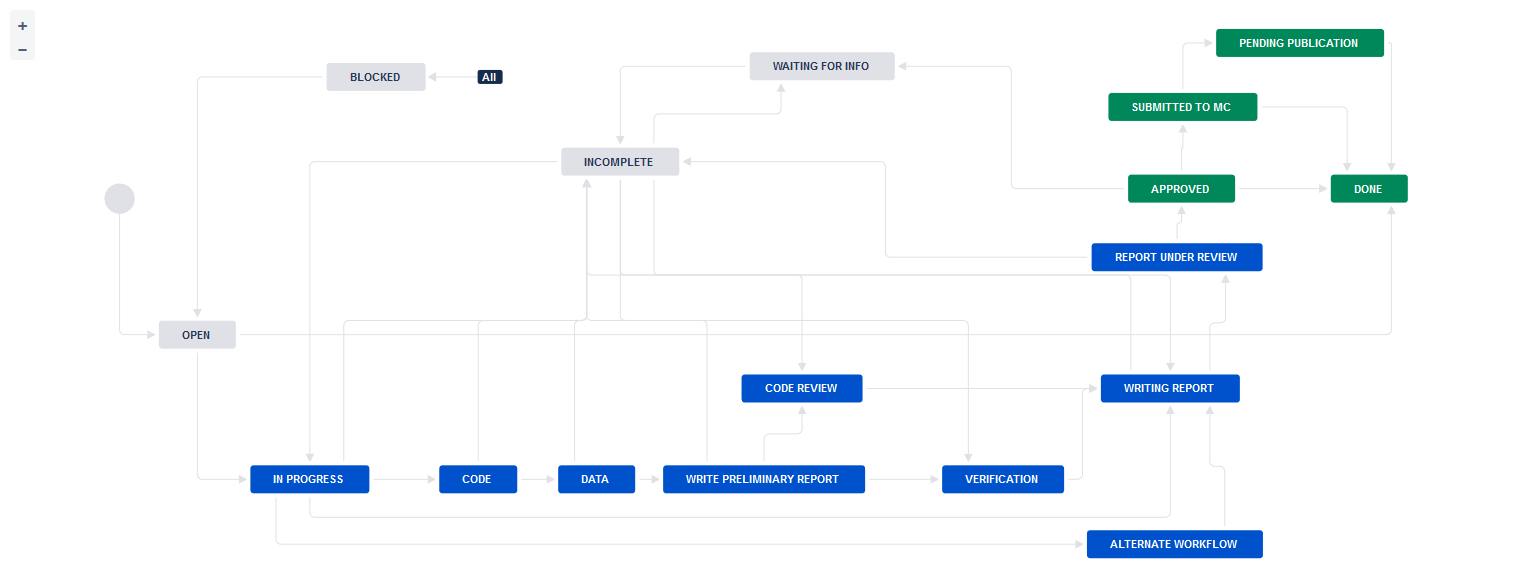
\includegraphics{images/AEADataEditorWorkflow-20191028.png}
\caption{Workflow stages}
\end{figure}

\hypertarget{raw-process-data}{%
\subsubsection{Raw process data}\label{raw-process-data}}

Raw process data is manually extracted from Jira, and saved as

\begin{itemize}
\tightlist
\item
  \texttt{export\_MM-DD-YYYY.csv} (for detailed transaction-level data)
\end{itemize}

The data is not made available outside of the organization, as it
contains names of replicators, manuscript numbers, and verbatim email
correspondence.

At this time, the latest extract was made 2022-12-08.

\hypertarget{anonymized-data}{%
\subsubsection{Anonymized data}\label{anonymized-data}}

We subset the raw data to variables of interest, and substitute random
numbers for sensitive strings. This is done by running
\texttt{01\_jira\_anonymize.R}. The programs saves both the confidential
version and the anonymized version.

\begin{Shaded}
\begin{Highlighting}[]
\FunctionTok{source}\NormalTok{(}\FunctionTok{file.path}\NormalTok{(programs,}\StringTok{"01\_jira\_anonymize.R"}\NormalTok{),}\AttributeTok{echo=}\ConstantTok{TRUE}\NormalTok{)}
\end{Highlighting}
\end{Shaded}

\begin{verbatim}
## 
## > rm(list = ls())
## 
## > gc()
##           used (Mb) gc trigger (Mb) max used (Mb)
## Ncells  825495 44.1    1412927 75.5  1412927 75.5
## Vcells 1498145 11.5    8388608 64.0  2372351 18.1
## 
## > source(here::here("programs", "config.R"), echo = TRUE)
## 
## > process_raw <- TRUE
## 
## > download_raw <- TRUE
## 
## > extractday <- "12-12-2022"
## 
## > firstday <- "2021-12-01"
## 
## > lastday <- "2022-11-30"
## 
## > basepath <- here::here()
## 
## > setwd(basepath)
## 
## > jiraconf <- file.path(basepath, "data", "confidential")
## 
## > if (Sys.getenv("HOSTNAME") == "zotique3") {
## +     jiraconf <- paste0(Sys.getenv("XDG_RUNTIME_DIR"), "/gvfs/dav:host=dav.box.com,ssl=true/dav/Office  ..." ... [TRUNCATED] 
## 
## > jiraanon <- file.path(basepath, "data", "anon")
## 
## > jirameta <- file.path(basepath, "data", "metadata")
## 
## > images <- file.path(basepath, "images")
## 
## > tables <- file.path(basepath, "tables")
## 
## > programs <- file.path(basepath, "programs")
## 
## > temp <- file.path(basepath, "data", "temp")
## 
## > for (dir in list(images, tables, programs, temp)) {
## +     if (file.exists(dir)) {
## +     }
## +     else {
## +         dir.create(file.path(dir))
## +     }
##  .... [TRUNCATED] 
## 
## > mran.date <- "2022-04-22"
## 
## > options(repos = paste0("https://cran.microsoft.com/snapshot/", 
## +     mran.date, "/"))
## 
## > pkgTest <- function(x) {
## +     if (!require(x, character.only = TRUE)) {
## +         install.packages(x, dep = TRUE)
## +         if (!require(x, charact .... [TRUNCATED] 
## 
## > pkgTest.github <- function(x, source) {
## +     if (!require(x, character.only = TRUE)) {
## +         install_github(paste(source, x, sep = "/"))
## +      .... [TRUNCATED] 
## 
## > if (file.exists(here::here("programs", "confidential-config.R"))) {
## +     source(here::here("programs", "confidential-config.R"))
## + }
## 
## > global.libraries <- c("dplyr", "tidyr", "splitstackshape")
## 
## > results <- sapply(as.list(global.libraries), pkgTest)
\end{verbatim}

\begin{verbatim}
## Loading required package: splitstackshape
\end{verbatim}

\begin{verbatim}
## 
## > exportfile <- paste0("export_", extractday, ".csv")
## 
## > if (!file.exists(file.path(jiraconf, exportfile))) {
## +     process_raw = FALSE
## +     print("Input file for anonymization not found - setting global  ..." ... [TRUNCATED] 
## [1] "Input file for anonymization not found - setting global parameter to FALSE"
## 
## > if (process_raw == TRUE) {
## +     jira.conf.raw <- read.csv(file.path(jiraconf, exportfile), 
## +         stringsAsFactors = FALSE) %>% rename(ticket = .... [TRUNCATED] 
## [1] "Not processing anonymization due to global parameter."
\end{verbatim}

\hypertarget{publishing-data}{%
\subsubsection{Publishing data}\label{publishing-data}}

Some additional cleaning and matching, and then we write out the file

\begin{Shaded}
\begin{Highlighting}[]
\FunctionTok{source}\NormalTok{(}\FunctionTok{file.path}\NormalTok{(programs,}\StringTok{"02\_jira\_anon\_publish.R"}\NormalTok{),}\AttributeTok{echo=}\ConstantTok{TRUE}\NormalTok{)}
\end{Highlighting}
\end{Shaded}

\begin{verbatim}
## 
## > source(here::here("programs", "config.R"), echo = TRUE)
## 
## > process_raw <- TRUE
## 
## > download_raw <- TRUE
## 
## > extractday <- "12-12-2022"
## 
## > firstday <- "2021-12-01"
## 
## > lastday <- "2022-11-30"
## 
## > basepath <- here::here()
## 
## > setwd(basepath)
## 
## > jiraconf <- file.path(basepath, "data", "confidential")
## 
## > if (Sys.getenv("HOSTNAME") == "zotique3") {
## +     jiraconf <- paste0(Sys.getenv("XDG_RUNTIME_DIR"), "/gvfs/dav:host=dav.box.com,ssl=true/dav/Office  ..." ... [TRUNCATED] 
## 
## > jiraanon <- file.path(basepath, "data", "anon")
## 
## > jirameta <- file.path(basepath, "data", "metadata")
## 
## > images <- file.path(basepath, "images")
## 
## > tables <- file.path(basepath, "tables")
## 
## > programs <- file.path(basepath, "programs")
## 
## > temp <- file.path(basepath, "data", "temp")
## 
## > for (dir in list(images, tables, programs, temp)) {
## +     if (file.exists(dir)) {
## +     }
## +     else {
## +         dir.create(file.path(dir))
## +     }
##  .... [TRUNCATED] 
## 
## > mran.date <- "2022-04-22"
## 
## > options(repos = paste0("https://cran.microsoft.com/snapshot/", 
## +     mran.date, "/"))
## 
## > pkgTest <- function(x) {
## +     if (!require(x, character.only = TRUE)) {
## +         install.packages(x, dep = TRUE)
## +         if (!require(x, charact .... [TRUNCATED] 
## 
## > pkgTest.github <- function(x, source) {
## +     if (!require(x, character.only = TRUE)) {
## +         install_github(paste(source, x, sep = "/"))
## +      .... [TRUNCATED] 
## 
## > global.libraries <- c("dplyr", "tidyr", "splitstackshape")
## 
## > results <- sapply(as.list(global.libraries), pkgTest)
## 
## > jira.anon.raw <- readRDS(file.path(jiraanon, "temp.jira.anon.RDS")) %>% 
## +     rename(reason.failure = Reason.for.Failure.to.Fully.Replicate) %>% 
## + .... [TRUNCATED] 
## 
## > jira.conf.subtask <- jira.anon.raw %>% select(ticket, 
## +     subtask) %>% cSplit("subtask", ",") %>% distinct() %>% pivot_longer(!ticket, 
## +     nam .... [TRUNCATED] 
## 
## > jira.anon <- jira.anon.raw %>% select(ticket, mc_number_anon) %>% 
## +     distinct(ticket, .keep_all = TRUE) %>% filter(mc_number_anon != 
## +     is.n .... [TRUNCATED]
\end{verbatim}

\begin{verbatim}
## Joining, by = "ticket"
\end{verbatim}

\begin{verbatim}
## 
## > saveRDS(jira.anon, file = file.path(jiraanon, "jira.anon.RDS"))
## 
## > write.csv(jira.anon, file = file.path(jiraanon, "jira.anon.csv"))
\end{verbatim}

\hypertarget{describing-the-data}{%
\subsection{Describing the Data}\label{describing-the-data}}

The anonymized data has 15 columns.

\hypertarget{variables}{%
\subsubsection{Variables}\label{variables}}

\begin{verbatim}
## Rows: 15 Columns: 2
## -- Column specification --------------------------------------------------------
## Delimiter: ","
## chr (2): name, label
## 
## i Use `spec()` to retrieve the full column specification for this data.
## i Specify the column types or set `show_col_types = FALSE` to quiet this message.
\end{verbatim}

\begin{longtable}[]{@{}
  >{\raggedright\arraybackslash}p{(\columnwidth - 2\tabcolsep) * \real{0.1011}}
  >{\raggedright\arraybackslash}p{(\columnwidth - 2\tabcolsep) * \real{0.8989}}@{}}
\toprule()
\begin{minipage}[b]{\linewidth}\raggedright
name
\end{minipage} & \begin{minipage}[b]{\linewidth}\raggedright
label
\end{minipage} \\
\midrule()
\endhead
ticket & The tracking number within the system. Project specific.
Sequentially assigned upon receipt. \\
date\_created & Date of a receipt \\
date\_updated & Date of a transaction \\
mc\_number\_anon & The (anonymized) number assigned by the editorial
workflow system (Manuscript Central/ ScholarOne) to a manuscript. This
is purged by a script of any revision suffixes. \\
Journal & Journal associated with an issue and manuscript. Derived from
the manuscript number. Possibly updated by hand \\
Status & Status associated with a ticket at any point in time. The
schema for these has changed over time. \\
Software.used & A list of software used to replicate the issue. \\
received & An indicator for whether the issue is just created and has
not been assigned to a replicator yet. \\
Changed.Fields & A transaction will change various fields. These are
listed here. \\
external & An indicator for whether the issue required the external
validation. \\
subtask & An indicator for whether the issue is a subtask of another
task. \\
Resolution & Resolution associated with a ticket at the end of the
replication process. \\
reason.failure & A list of reasons for failure to fully replicate. \\
MCRecommendation & Decision status when the issue is Revise and
Resubmit. \\
MCRecommendationV2 & Decision status when the issue is conditionally
accepted. \\
\bottomrule()
\end{longtable}

\hypertarget{sample-records}{%
\subsubsection{Sample records}\label{sample-records}}

\begin{longtable}[]{@{}
  >{\raggedright\arraybackslash}p{(\columnwidth - 28\tabcolsep) * \real{0.0553}}
  >{\raggedright\arraybackslash}p{(\columnwidth - 28\tabcolsep) * \real{0.0599}}
  >{\raggedright\arraybackslash}p{(\columnwidth - 28\tabcolsep) * \real{0.0599}}
  >{\raggedleft\arraybackslash}p{(\columnwidth - 28\tabcolsep) * \real{0.0691}}
  >{\raggedright\arraybackslash}p{(\columnwidth - 28\tabcolsep) * \real{0.0922}}
  >{\raggedright\arraybackslash}p{(\columnwidth - 28\tabcolsep) * \real{0.0323}}
  >{\raggedright\arraybackslash}p{(\columnwidth - 28\tabcolsep) * \real{0.0645}}
  >{\raggedright\arraybackslash}p{(\columnwidth - 28\tabcolsep) * \real{0.0415}}
  >{\raggedright\arraybackslash}p{(\columnwidth - 28\tabcolsep) * \real{0.1382}}
  >{\raggedright\arraybackslash}p{(\columnwidth - 28\tabcolsep) * \real{0.0415}}
  >{\raggedright\arraybackslash}p{(\columnwidth - 28\tabcolsep) * \real{0.0369}}
  >{\raggedright\arraybackslash}p{(\columnwidth - 28\tabcolsep) * \real{0.0737}}
  >{\raggedright\arraybackslash}p{(\columnwidth - 28\tabcolsep) * \real{0.0691}}
  >{\raggedright\arraybackslash}p{(\columnwidth - 28\tabcolsep) * \real{0.0783}}
  >{\raggedright\arraybackslash}p{(\columnwidth - 28\tabcolsep) * \real{0.0876}}@{}}
\toprule()
\begin{minipage}[b]{\linewidth}\raggedright
ticket
\end{minipage} & \begin{minipage}[b]{\linewidth}\raggedright
date\_created
\end{minipage} & \begin{minipage}[b]{\linewidth}\raggedright
date\_updated
\end{minipage} & \begin{minipage}[b]{\linewidth}\raggedleft
mc\_number\_anon
\end{minipage} & \begin{minipage}[b]{\linewidth}\raggedright
Journal
\end{minipage} & \begin{minipage}[b]{\linewidth}\raggedright
Status
\end{minipage} & \begin{minipage}[b]{\linewidth}\raggedright
Software.used
\end{minipage} & \begin{minipage}[b]{\linewidth}\raggedright
received
\end{minipage} & \begin{minipage}[b]{\linewidth}\raggedright
Changed.Fields
\end{minipage} & \begin{minipage}[b]{\linewidth}\raggedright
external
\end{minipage} & \begin{minipage}[b]{\linewidth}\raggedright
subtask
\end{minipage} & \begin{minipage}[b]{\linewidth}\raggedright
Resolution
\end{minipage} & \begin{minipage}[b]{\linewidth}\raggedright
reason.failure
\end{minipage} & \begin{minipage}[b]{\linewidth}\raggedright
MCRecommendation
\end{minipage} & \begin{minipage}[b]{\linewidth}\raggedright
MCRecommendationV2
\end{minipage} \\
\midrule()
\endhead
AEAREP-3787 & 2022-12-08 & 2022-12-08 & 1316 & AEJ:Economic Policy &
Open & Stata,R & No & Software used & No & NA & & & & \\
AEAREP-3787 & 2022-12-08 & 2022-12-08 & 1316 & AEJ:Economic Policy &
Open & & No & openICPSR Project Number & No & NA & & & & \\
AEAREP-3787 & 2022-12-08 & 2022-12-08 & 1316 & AEJ:Economic Policy &
Open & & NA & Manuscript Central identifier & No & NA & & & & \\
AEAREP-3787 & 2022-12-08 & 2022-12-08 & 1316 & AEJ:Economic Policy &
Open & & NA & Journal & No & NA & & & & \\
AEAREP-3787 & 2022-12-08 & 2022-12-08 & 1316 & & Open & & NA & & No & NA
& & & & \\
AEAREP-3786 & 2022-12-07 & 2022-12-07 & 316 & AER & Done & & No & Status
& No & NA & Evaluation only & & & \\
\bottomrule()
\end{longtable}

\hypertarget{lab-members-during-this-period}{%
\subsubsection{Lab members during this
period}\label{lab-members-during-this-period}}

We list the lab members active at some point during this period.

\begin{Shaded}
\begin{Highlighting}[]
\FunctionTok{source}\NormalTok{(}\FunctionTok{file.path}\NormalTok{(programs,}\StringTok{"03\_lab\_members.R"}\NormalTok{),}\AttributeTok{echo=}\ConstantTok{TRUE}\NormalTok{)}
\end{Highlighting}
\end{Shaded}

\begin{verbatim}
## 
## > rm(list = ls())
## 
## > gc()
##           used (Mb) gc trigger  (Mb) max used  (Mb)
## Ncells  988576 52.8    1866287  99.7  1866287  99.7
## Vcells 1897560 14.5   24597022 187.7 30746277 234.6
## 
## > source(here::here("programs", "config.R"), echo = TRUE)
## 
## > process_raw <- TRUE
## 
## > download_raw <- TRUE
## 
## > extractday <- "12-12-2022"
## 
## > firstday <- "2021-12-01"
## 
## > lastday <- "2022-11-30"
## 
## > basepath <- here::here()
## 
## > setwd(basepath)
## 
## > jiraconf <- file.path(basepath, "data", "confidential")
## 
## > if (Sys.getenv("HOSTNAME") == "zotique3") {
## +     jiraconf <- paste0(Sys.getenv("XDG_RUNTIME_DIR"), "/gvfs/dav:host=dav.box.com,ssl=true/dav/Office  ..." ... [TRUNCATED] 
## 
## > jiraanon <- file.path(basepath, "data", "anon")
## 
## > jirameta <- file.path(basepath, "data", "metadata")
## 
## > images <- file.path(basepath, "images")
## 
## > tables <- file.path(basepath, "tables")
## 
## > programs <- file.path(basepath, "programs")
## 
## > temp <- file.path(basepath, "data", "temp")
## 
## > for (dir in list(images, tables, programs, temp)) {
## +     if (file.exists(dir)) {
## +     }
## +     else {
## +         dir.create(file.path(dir))
## +     }
##  .... [TRUNCATED] 
## 
## > mran.date <- "2022-04-22"
## 
## > options(repos = paste0("https://cran.microsoft.com/snapshot/", 
## +     mran.date, "/"))
## 
## > pkgTest <- function(x) {
## +     if (!require(x, character.only = TRUE)) {
## +         install.packages(x, dep = TRUE)
## +         if (!require(x, charact .... [TRUNCATED] 
## 
## > pkgTest.github <- function(x, source) {
## +     if (!require(x, character.only = TRUE)) {
## +         install_github(paste(source, x, sep = "/"))
## +      .... [TRUNCATED] 
## 
## > global.libraries <- c("dplyr", "tidyr", "splitstackshape")
## 
## > results <- sapply(as.list(global.libraries), pkgTest)
## 
## > jira.conf.plus <- readRDS(file = file.path(jiraconf, 
## +     "jira.conf.plus.RDS"))
## 
## > lab.member <- jira.conf.plus %>% filter(Change.Author != 
## +     "" & Change.Author != "Automation for Jira" & Change.Author != 
## +     "LV (Data Edit ..." ... [TRUNCATED] 
## 
## > write.table(lab.member, file = file.path(basepath, 
## +     "data", "replicationlab_members.txt"), sep = "\t", row.names = FALSE)
## 
## > external.member <- jira.conf.plus %>% filter(External.party.name != 
## +     "") %>% mutate(date_created = as.Date(substr(Created, 1, 
## +     10), "%m/ ..." ... [TRUNCATED] 
## 
## > write.table(external.member, file = file.path(basepath, 
## +     "data", "external_replicators.txt"), sep = "\t", row.names = FALSE)
\end{verbatim}

There were a total of 42 lab members over the course of the 12 month
period.

\hypertarget{r-session-info}{%
\subsubsection{R session info}\label{r-session-info}}

\begin{Shaded}
\begin{Highlighting}[]
\FunctionTok{sessionInfo}\NormalTok{()}
\end{Highlighting}
\end{Shaded}

\begin{verbatim}
## R version 4.2.2 (2022-10-31)
## Platform: x86_64-pc-linux-gnu (64-bit)
## Running under: Ubuntu 22.04.1 LTS
## 
## Matrix products: default
## BLAS:   /usr/lib/x86_64-linux-gnu/openblas-pthread/libblas.so.3
## LAPACK: /usr/lib/x86_64-linux-gnu/openblas-pthread/libopenblasp-r0.3.20.so
## 
## locale:
##  [1] LC_CTYPE=en_US.UTF-8       LC_NUMERIC=C              
##  [3] LC_TIME=en_US.UTF-8        LC_COLLATE=en_US.UTF-8    
##  [5] LC_MONETARY=en_US.UTF-8    LC_MESSAGES=en_US.UTF-8   
##  [7] LC_PAPER=en_US.UTF-8       LC_NAME=C                 
##  [9] LC_ADDRESS=C               LC_TELEPHONE=C            
## [11] LC_MEASUREMENT=en_US.UTF-8 LC_IDENTIFICATION=C       
## 
## attached base packages:
## [1] stats     graphics  grDevices utils     datasets  methods   base     
## 
## other attached packages:
## [1] splitstackshape_1.4.8 readr_2.1.3           knitr_1.41           
## [4] tidyr_1.2.1           stringr_1.5.0         dplyr_1.0.10         
## 
## loaded via a namespace (and not attached):
##  [1] highr_0.9         pillar_1.8.1      compiler_4.2.2    tools_4.2.2      
##  [5] bit_4.0.5         digest_0.6.30     evaluate_0.18     lifecycle_1.0.3  
##  [9] tibble_3.1.8      pkgconfig_2.0.3   rlang_1.0.6       cli_3.4.1        
## [13] DBI_1.1.3         rstudioapi_0.14   parallel_4.2.2    yaml_2.3.6       
## [17] xfun_0.39         fastmap_1.1.0     withr_2.5.0       generics_0.1.3   
## [21] vctrs_0.5.1       hms_1.1.2         bit64_4.0.5       rprojroot_2.0.3  
## [25] tidyselect_1.2.0  glue_1.6.2        data.table_1.14.6 here_1.0.1       
## [29] R6_2.5.1          fansi_1.0.3       vroom_1.6.0       rmarkdown_2.18   
## [33] purrr_0.3.5       tzdb_0.3.0        magrittr_2.0.3    htmltools_0.5.4  
## [37] ellipsis_0.3.2    assertthat_0.2.1  utf8_1.2.2        stringi_1.7.8    
## [41] crayon_1.5.2
\end{verbatim}

\end{document}
